% vim:tw=60

\section{Experiences}
\label{sec:exp}

\notes{any rational? What is the point? It is effective on
what? and why}

\subsection{Understanding runtime behaviour}

We try to use the mined data hierarchy from logs to
understand runtime behaviour of cosmos client and EN server.
Cosmos is a distributed storage system similiar to GFS. The
EN server is similiar to the role of chunkserver. In cosmos,
data is organized in streams and streams are comprised of
extents. Each stream and extent is identified by a GUID.

We choose (Session, opId) to analyze cosmos client runtime
and choose ExtentID to analyze EN server runtime.

At the client side, we upload several files into cosmos and
query the streams status. We apply task model Session $:=$
opId$+$ on cosmos client log to investigate its runtime
behaviour. We successfully divide the activities of each
threads by Session and Opid.

There is one client thread who receives user commands and
each command is run as a session. A command is executed in
steps as different opId. Within a opId, it issues several
RPC calls. The client thread does not run the RPC calls, but
puts them into a queue. Other threads are workers who get
RPC calls and run them. When the responses for RPC calls are
returned, the workers notify the client threads on the
results. The workers does not know the session concept and
their activities are divided by opIds. The client and worker
threads activities can be connected by the same opId.

\begin{figure}
\centering
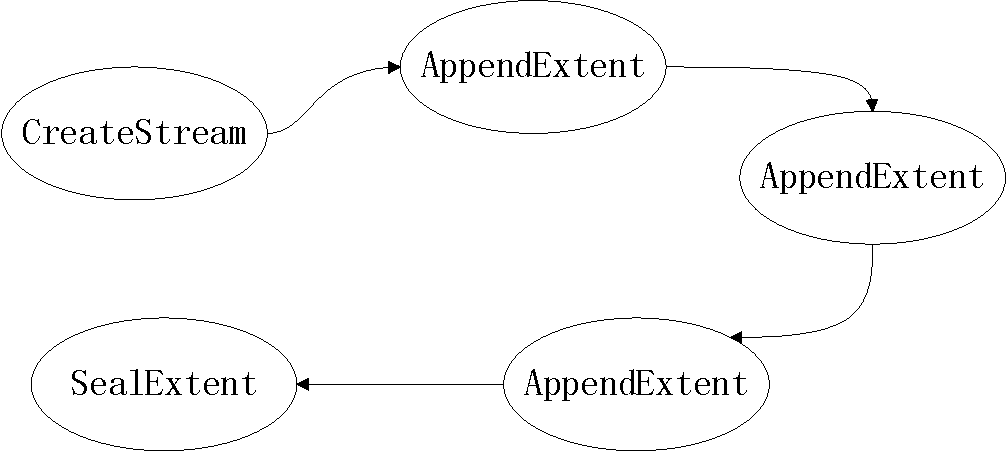
\includegraphics[height=1.5in]{clientcreate}
\caption{The process of create a stream at client side.}
\label{fig:clientcreate}
\end{figure}

We look at how a file is uploaded into cosmos as stream
specifically. The process of create a stream at client side
is executed as four opIds and six RPC commands, as shown in
Figure~\ref{fig:clientcreate}. They are (create a stream),
(append stream, append extent), (append extent), (append
extent and seal the extent). Each parentheses indicate a
different opId. As the file size is smaller than the maximux
allowed extent size, the created stream contains only one
extent, and its content is sent by three append RPC calls.
After the last appending extent request, the extent is
sealed and no further append is allowed.

\begin{figure}
\centering
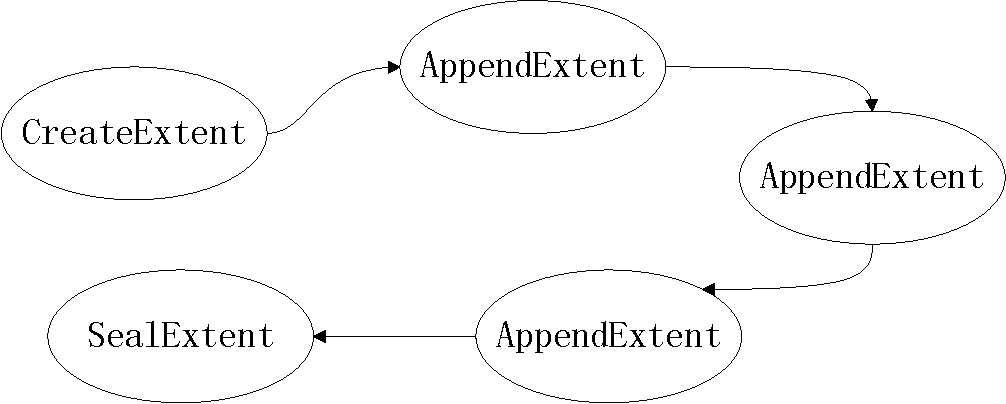
\includegraphics[height=1.5in]{encreate}
\caption{Create and append extent at EN side.}
\label{fig:encreate}
\end{figure}

We then investigae the corresponding activities at EN side.
The result is shown in Figure~\ref{fig:encreate}. There
are five RPC calls handled by the same thread. They are
create extent, three append extent and seal extent. Using
ExtentID, we can only distinguish at extent operation level,
so the five RPC handling process are treated as one task
instance.

\lesson Using task models translated from data hierarchy, we
can effectively identify task instances and understanding
system runtime behaviour. The advantage is, data
hierarchy is predefined by system design and the result
should be more precise than bottom-up mining.

Another property is that we can see how high leve task is
translated into several low level sub-task.

\comment{
We apply our task model to understanding runtime behaviour
for each thread. To obtaining the whole execution path for
handling a request, we have to asscociate task instances
with causal dependencies.

Our technique is complementary to
existing ones in that 

we can combine scalpel and data hierarchy together. Using
scalpel to automatically find dependency, and use data
hierarchy to find task boundary. 
}

There are some disadvantages. First the boundary of task
instances may have a phase shift. The initialization part of
a task instance doesn't know the data identifer yet so it
will be merged into the tail of previous task instances.
However, as initialization is relatively static and this
phase shift can be corrected by adding a predefined
displacement to task boundaries. Second, the granularity of
task observed depends on the choice of keys. As demonstrated
in EN server, several RPC handling task is merged into one
task because they happpens to handle the same extent.

\subsection{Guide on debugging}

We then show how we use the task model to help find a
performace problem in cosmos.

It is reported from tester that the cosmos network library
cannot go through a bandwidth stress test. In the test,
it uses several threads to concurrently issue RPC calls of
fixed size (typically 128KB) and see whether the bandwidth
is fully saturated. The result is negative, the bandwidth is
only about 34\% of its capability, while the CPU usage is
far under 100\%.

To our experiences, performance bugs are usually caused by
convoluted application logic within deep code base. We try
to use task model to find hints and narrow down the bug site
as far as possible.

\begin{figure}
\centering
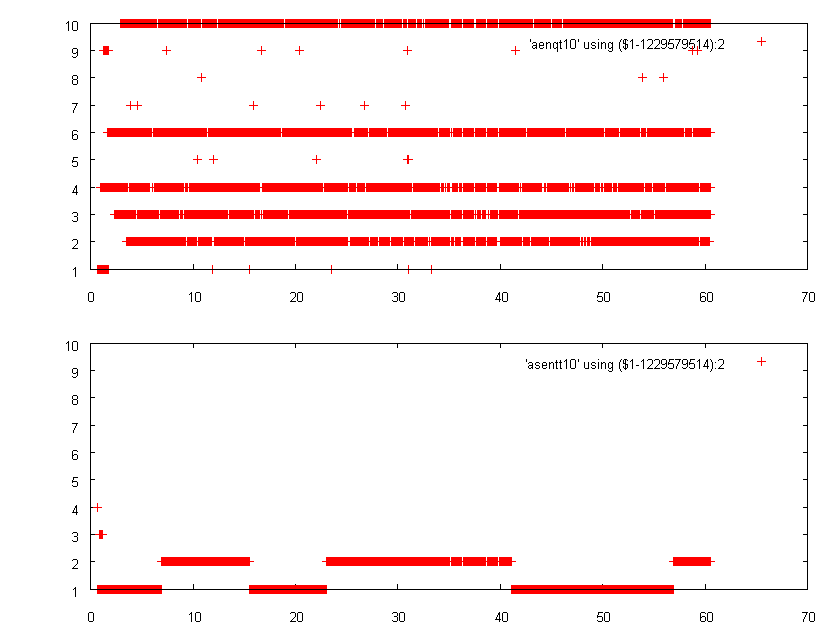
\includegraphics[height=2.4in]{stresstest}
\caption{Task trace for stress test}
\label{fig:stresstest}
\end{figure}

We repeat the stress test and collect timing of each task
instances. Figure~\ref{fig:stresstest} shows the the overall
picture of task traces.

We can immediately see from the figure that the worker
threads are highly suspicious. They work in a synchronized
way and non of worker threads' task instances have overlap
with others.

By examining cosmos worker's processing model, we finally
find the root cause. When a worker thread get a RPC message
from queue, it uses a processor object to process the
message. However, all worker threads share one processor for
each connection. Thus the processor object becomes a scarce
resource which force worker threads work serially.

\lesson Task model is very useful for narrowing down bug
sites and helps reasoning about the root cause. With proper
visualization, we can summarize the pattern for bugs. It is
expected that performance bug have limited kinds of causes
and each of them maps to different bug patterns. We can use
the reverse mapping from a spotted bug pattern to determine
it root cause.

A lot of performance bugs are caused by resource
contentions. The resource can be CPU, I/O, or mutex and
shared object (processor object in above case). With proper
helps (static analysis, instrumentation, etc.) we can
summarize the set of resources shared by tasks, analyze
their contention condition and shoot the root cause of
performance problems precisely.

